\specialsection{Масштабирование участников видеоконференций}

Хотя WebRTC представляет собой мощный интрумент для решения многих проблем при создании системы видеоконференций - он не идеален. Фреймворк WebRTC был разработан с учетом одноранговой (P2P) архитектуры, такой подход имеет проблемы с масштабируюмостью, если мы хотим одновременное присутствие большого количества участников. В WebRTC общающиеся стороны должны кодировать отдельный поток для получателей. Таким образом, каждый получатель связан независимым и выделенным кодером на стороне отправителя. Для поддержки N участников конференции с помощью чистой Mesh сети потребуется N * (N - 1) / 2 каналов. То есть требования к пропускной способности устройств будет расти квадратично по отношению к числу участников видеоконференции, рис ~\ref{mesh} \cite{v17}.

\begin{figure}[ht]
\begin{center}
\scalebox{0.30}{
   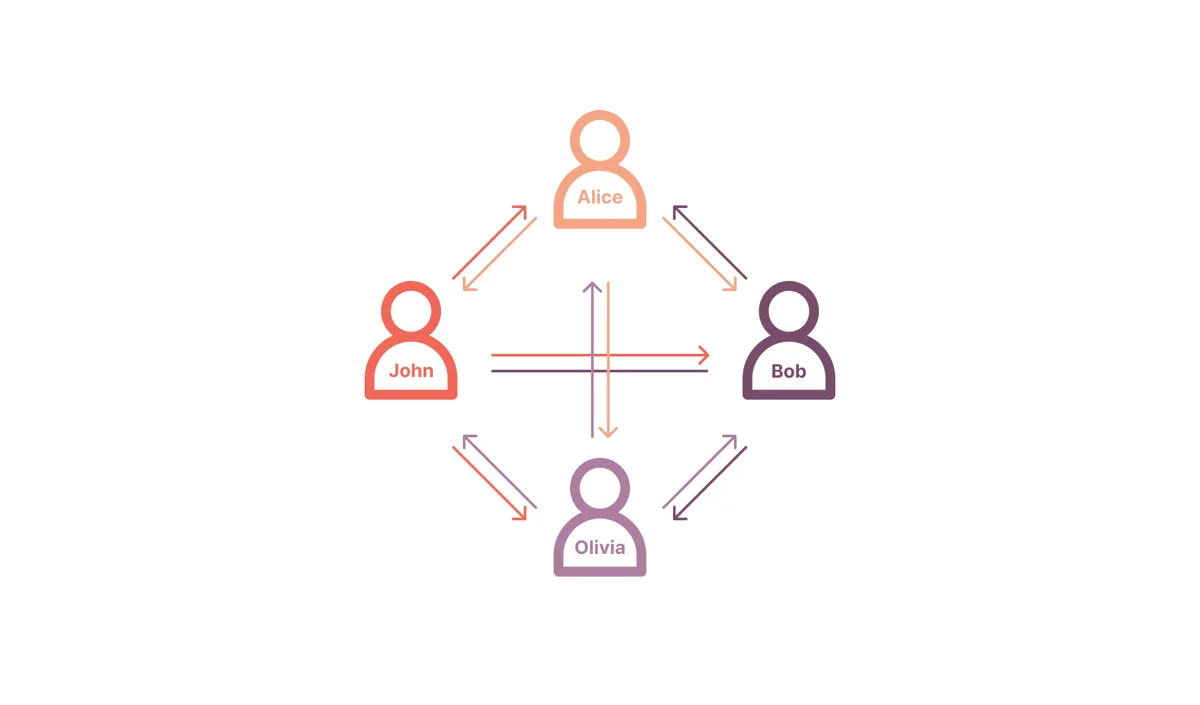
\includegraphics{images/mesh.png}
}

\caption{
\label{mesh}
     Mesh архитектура.}
\end {center}
\end {figure}

Чтобы улучшить масштабируемость этой архитектуры, можно использовать промежуточный медиасервер. В WebRTC есть 2 распространенных подхода - использование устройства многоточечной конференции (MCU) или устройства селективной переадресации (SFU).

\specialsubsection{SFU}

В WebRTC функции контроллера конференции может выполнять устройство селективной переадресации (SFU), задачей которого является получение всех потоков и принятие решения о том, какой поток должен быть отправлен какому участнику. Задача контроллера - оптимизация доставки потоков реального времени от отправителя к получателю.

В отличие от подхода MCU, SFU не требует декодирования/кодирования и поэтому является более легким. Его основная задача это принимать все потоки от участников и выборочно пересылать один или несколько потоков каждому получателю, рис. ~\ref{sfu}.

\begin{figure}[ht]
\begin{center}
\scalebox{0.50}{
   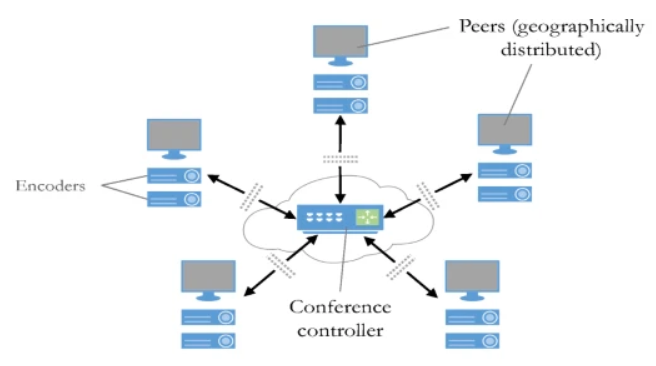
\includegraphics{images/sfu.png}
}

\caption{
\label{sfu}
     SFU архитектура.}
\end {center}
\end {figure}

При большом количестве участников количество пересылаемых потоков необходимо ограничивать, чтобы не тратить пропускную способность. По этой причине Грозева и др. разработали алгоритм идентификации докладчиков, который определит N последних доминирующих докладчиков конференции. Для экономии полосы пропускания только эти N потоков передаются участникам видеоконференции.

\begin{figure}[ht]
\begin{center}
\scalebox{0.50}{
   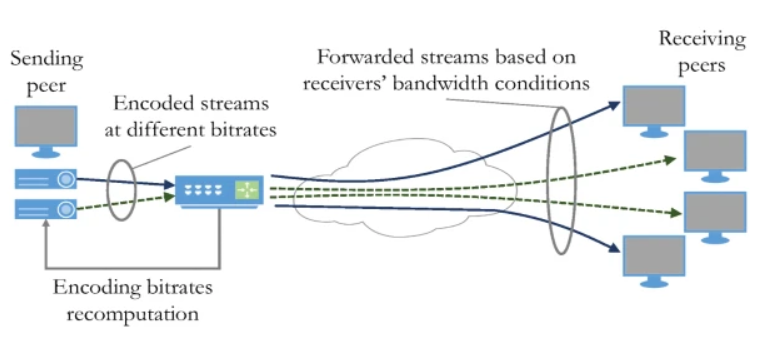
\includegraphics{images/sfu_forwarding.png}
}

\caption{
\label{sfu-forwarding}
     SFU controller dynamic forwarding.}
\end {center}
\end {figure}

По сути контроллер выполняет 2 основные задачи:
\begin{itemize}
	\item[1.] Получает все кодированные потоки от отправителя и динамически направляет их получателям, исходя из доступной пропускной способности, рис. ~\ref{sfu-forwarding};
	\item[2.] Переодически пересчитывает битрейты кодирования отправителя, чтобы лучше следовать долгосрочным колебаниям сети получателя \cite{v18}.
\end{itemize}

\specialsubsection{MCU}

Подход MCU заключается в том, чтобы получить все потоки от участников, декодировать и компилировать их в один общий поток, который отправляется обратно участникам. В итоге каждый участник должен отправлять и получать только один поток. Стоит понимать, что операции MCU дорогостоящие и требуют больших вычислительных затрат из процессов декодирования-смешивания-кодирования.

\begin{figure}[ht]
\begin{center}
\scalebox{0.90}{
   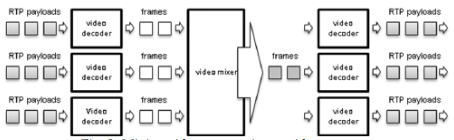
\includegraphics{images/mcu.png}
}

\caption{
\label{mcu}
     MCU смешивание аудиопотоков.}
\end {center}
\end {figure}

MCU назначает аудио/видео кодер и декодер, которые способны декодировать RTP-потоки от участников, кодер кодирует смешанные видеокадры обратно в полезную нагрузку RTP для каждого участника. Простое смешивание аудиопотоков всех участников в один поток привело бы к появлению эха от голоса. Чтобы этого избежать каждый участник должен иметь собственный аудиопоток, который не содержит его собственного звука. Сначала аудиокодеры декодируют полезную нагрузку RTP в аудиообразцы. Затем аудиомикшер смешивает аудиообразцы в отдельные потоки аудиообразцов, как показано на рис. ~\ref{mcu}. Потом отдельный аудиокодер кодирует аудиообразцы обратно в полезную нагрузку RTP \cite{v19}.

\specialsubsection{Сравнение архитектур}

\begin{center}
    \begin{longtable}{|p{4cm}|p{3cm}|p{3cm}|p{3cm}|}
    \caption{Сравнение Mesh, MCU, SFU архитектур.}\\
    \hline
     & Mesh & MCU & SFU\\ 
    \hline 
    in/out streams & 3/3 & 1/1 & 3/1\\
    \hline
    input traffic & 3 Мбит/с & 1 Мбит/с & 3 Мбит/с\\
    \hline
    output traffic & 3 Мбит/с & 1 Мбит/с & 1 Мбит/с\\
    \hline
    client CPU & 3 encoder + 3 decoder = 60\% & 1 encoder + 1 decoder = 20\% & 1 encoder + 3 decoder = 40\%\\
    \hline
    server CPU & 0 & 100\% & 10\%\\
    \hline
    latency & min & max & avg\\
    \hline
    SIP/live & -- & + & --\\
    \hline
    max participants & ~8 & $\infty$ & ~50\\
    \hline
    \end{longtable}
\end{center}

\specialsubsection{Mesh}

Mesh-топология выгодна за счет прямого соединения участников без вмешательства сервера, что сокращает издержки. 

Однако с ростом числа участников квадратично растет входящий и исходящий трафик. Создается большая нагрузка на CPU клиентского устройства, потому что большинство устройств поддерживают аппаратно ускоренное кодирование только одного потока в один момент, а тут надо кодировать и декодировать сразу несколько потоков.

\specialsubsection{MCU}

Основное преимущество MCU - число участников ограничено только количеством потоков, которое можно смикшировать на сервере. Кроме того, MCU экономит ресурсы на клиенте и позволяет реализовать трансляцию или запись на сервере.

Однако в MCU требуется много ресурсов на сервере, а также задержка в этой архитектуре самая большая.

\specialsubsection{SFU}

SFU архитектура выгодна за счет того, что часть нагрузки переносится с сервера на клиент. Кроме того исходящий трафик постоянен, а входящий растет пропорционально числу участников видеоконференции.

Главный минус SFU - это ограниченное число максимальных участников, которое, конечно, выше, чем в Mesh архитектуре, но меньше, чем в MCU. Это происходит из-за дорогого микширования входящих потоков, которое ложится на клиентов \cite{v20}.

\pagebreak